\documentclass[conference]{IEEEtran}
\usepackage{cite}
\usepackage{amsmath,amssymb,amsfonts}
\usepackage{graphicx}
\usepackage{textcomp}
\usepackage{xcolor}
\usepackage{url}
\usepackage{booktabs}
\usepackage[hidelinks,breaklinks=true]{hyperref}

% Input the automated results summary macros
%% Automated results summary generated by generate_latex_results.py
%% Do not edit manually!

\newcommand{\pretrainedfrozenValEpochsMean}{8.0}
\newcommand{\pretrainedfrozenValEpochsStd}{0.8}
\newcommand{\pretrainedfrozenValAccMean}{93.82\%}
\newcommand{\pretrainedfrozenValAccStd}{0.32\%}
\newcommand{\pretrainedfrozenTestAccMean}{93.27\%}
\newcommand{\pretrainedfrozenTestAccStd}{0.23\%}
\newcommand{\pretrainedfrozenClosestSeed}{100}
\newcommand{\pretrainedfrozenRepPrecBuildings}{93.2\%}
\newcommand{\pretrainedfrozenRepRecBuildings}{93.4\%}
\newcommand{\pretrainedfrozenRepFBuildings}{93.3\%}
\newcommand{\pretrainedfrozenRepPrecForest}{98.7\%}
\newcommand{\pretrainedfrozenRepRecForest}{99.4\%}
\newcommand{\pretrainedfrozenRepFForest}{99.1\%}
\newcommand{\pretrainedfrozenRepPrecGlacier}{93.9\%}
\newcommand{\pretrainedfrozenRepRecGlacier}{82.8\%}
\newcommand{\pretrainedfrozenRepFGlacier}{88.0\%}
\newcommand{\pretrainedfrozenRepPrecMountain}{86.3\%}
\newcommand{\pretrainedfrozenRepRecMountain}{92.2\%}
\newcommand{\pretrainedfrozenRepFMountain}{89.1\%}
\newcommand{\pretrainedfrozenRepPrecSea}{95.1\%}
\newcommand{\pretrainedfrozenRepRecSea}{98.6\%}
\newcommand{\pretrainedfrozenRepFSea}{96.8\%}
\newcommand{\pretrainedfrozenRepPrecStreet}{93.3\%}
\newcommand{\pretrainedfrozenRepRecStreet}{94.4\%}
\newcommand{\pretrainedfrozenRepFStreet}{93.8\%}
\newcommand{\pretrainedfrozenRepAcc}{93.23\%}
\newcommand{\pretrainedfrozenCM}[2]{%
  \ifnum#1=0\relax\ifnum#2=0\relax{408}\fi\fi%
  \ifnum#1=0\relax\ifnum#2=1\relax{0}\fi\fi%
  \ifnum#1=0\relax\ifnum#2=2\relax{0}\fi\fi%
  \ifnum#1=0\relax\ifnum#2=3\relax{0}\fi\fi%
  \ifnum#1=0\relax\ifnum#2=4\relax{1}\fi\fi%
  \ifnum#1=0\relax\ifnum#2=5\relax{28}\fi\fi%
  \ifnum#1=1\relax\ifnum#2=0\relax{0}\fi\fi%
  \ifnum#1=1\relax\ifnum#2=1\relax{471}\fi\fi%
  \ifnum#1=1\relax\ifnum#2=2\relax{0}\fi\fi%
  \ifnum#1=1\relax\ifnum#2=3\relax{1}\fi\fi%
  \ifnum#1=1\relax\ifnum#2=4\relax{0}\fi\fi%
  \ifnum#1=1\relax\ifnum#2=5\relax{2}\fi\fi%
  \ifnum#1=2\relax\ifnum#2=0\relax{1}\fi\fi%
  \ifnum#1=2\relax\ifnum#2=1\relax{4}\fi\fi%
  \ifnum#1=2\relax\ifnum#2=2\relax{458}\fi\fi%
  \ifnum#1=2\relax\ifnum#2=3\relax{71}\fi\fi%
  \ifnum#1=2\relax\ifnum#2=4\relax{16}\fi\fi%
  \ifnum#1=2\relax\ifnum#2=5\relax{3}\fi\fi%
  \ifnum#1=3\relax\ifnum#2=0\relax{1}\fi\fi%
  \ifnum#1=3\relax\ifnum#2=1\relax{2}\fi\fi%
  \ifnum#1=3\relax\ifnum#2=2\relax{28}\fi\fi%
  \ifnum#1=3\relax\ifnum#2=3\relax{484}\fi\fi%
  \ifnum#1=3\relax\ifnum#2=4\relax{9}\fi\fi%
  \ifnum#1=3\relax\ifnum#2=5\relax{1}\fi\fi%
  \ifnum#1=4\relax\ifnum#2=0\relax{2}\fi\fi%
  \ifnum#1=4\relax\ifnum#2=1\relax{0}\fi\fi%
  \ifnum#1=4\relax\ifnum#2=2\relax{2}\fi\fi%
  \ifnum#1=4\relax\ifnum#2=3\relax{3}\fi\fi%
  \ifnum#1=4\relax\ifnum#2=4\relax{503}\fi\fi%
  \ifnum#1=4\relax\ifnum#2=5\relax{0}\fi\fi%
  \ifnum#1=5\relax\ifnum#2=0\relax{26}\fi\fi%
  \ifnum#1=5\relax\ifnum#2=1\relax{0}\fi\fi%
  \ifnum#1=5\relax\ifnum#2=2\relax{0}\fi\fi%
  \ifnum#1=5\relax\ifnum#2=3\relax{2}\fi\fi%
  \ifnum#1=5\relax\ifnum#2=4\relax{0}\fi\fi%
  \ifnum#1=5\relax\ifnum#2=5\relax{473}\fi\fi%
}
\newcommand{\randomfrozenValEpochsMean}{8.7}
\newcommand{\randomfrozenValEpochsStd}{2.1}
\newcommand{\randomfrozenValAccMean}{67.83\%}
\newcommand{\randomfrozenValAccStd}{4.62\%}
\newcommand{\randomfrozenTestAccMean}{66.54\%}
\newcommand{\randomfrozenTestAccStd}{4.04\%}
\newcommand{\randomfrozenClosestSeed}{100}
\newcommand{\randomfrozenRepPrecBuildings}{53.0\%}
\newcommand{\randomfrozenRepRecBuildings}{64.5\%}
\newcommand{\randomfrozenRepFBuildings}{58.2\%}
\newcommand{\randomfrozenRepPrecForest}{62.5\%}
\newcommand{\randomfrozenRepRecForest}{97.9\%}
\newcommand{\randomfrozenRepFForest}{76.3\%}
\newcommand{\randomfrozenRepPrecGlacier}{78.7\%}
\newcommand{\randomfrozenRepRecGlacier}{53.5\%}
\newcommand{\randomfrozenRepFGlacier}{63.7\%}
\newcommand{\randomfrozenRepPrecMountain}{67.1\%}
\newcommand{\randomfrozenRepRecMountain}{69.5\%}
\newcommand{\randomfrozenRepFMountain}{68.3\%}
\newcommand{\randomfrozenRepPrecSea}{76.4\%}
\newcommand{\randomfrozenRepRecSea}{49.4\%}
\newcommand{\randomfrozenRepFSea}{60.0\%}
\newcommand{\randomfrozenRepPrecStreet}{68.1\%}
\newcommand{\randomfrozenRepRecStreet}{64.7\%}
\newcommand{\randomfrozenRepFStreet}{66.3\%}
\newcommand{\randomfrozenRepAcc}{66.10\%}
\newcommand{\randomfrozenCM}[2]{%
  \ifnum#1=0\relax\ifnum#2=0\relax{282}\fi\fi%
  \ifnum#1=0\relax\ifnum#2=1\relax{64}\fi\fi%
  \ifnum#1=0\relax\ifnum#2=2\relax{0}\fi\fi%
  \ifnum#1=0\relax\ifnum#2=3\relax{11}\fi\fi%
  \ifnum#1=0\relax\ifnum#2=4\relax{7}\fi\fi%
  \ifnum#1=0\relax\ifnum#2=5\relax{73}\fi\fi%
  \ifnum#1=1\relax\ifnum#2=0\relax{4}\fi\fi%
  \ifnum#1=1\relax\ifnum#2=1\relax{464}\fi\fi%
  \ifnum#1=1\relax\ifnum#2=2\relax{0}\fi\fi%
  \ifnum#1=1\relax\ifnum#2=3\relax{1}\fi\fi%
  \ifnum#1=1\relax\ifnum#2=4\relax{0}\fi\fi%
  \ifnum#1=1\relax\ifnum#2=5\relax{5}\fi\fi%
  \ifnum#1=2\relax\ifnum#2=0\relax{64}\fi\fi%
  \ifnum#1=2\relax\ifnum#2=1\relax{29}\fi\fi%
  \ifnum#1=2\relax\ifnum#2=2\relax{296}\fi\fi%
  \ifnum#1=2\relax\ifnum#2=3\relax{86}\fi\fi%
  \ifnum#1=2\relax\ifnum#2=4\relax{33}\fi\fi%
  \ifnum#1=2\relax\ifnum#2=5\relax{45}\fi\fi%
  \ifnum#1=3\relax\ifnum#2=0\relax{41}\fi\fi%
  \ifnum#1=3\relax\ifnum#2=1\relax{41}\fi\fi%
  \ifnum#1=3\relax\ifnum#2=2\relax{36}\fi\fi%
  \ifnum#1=3\relax\ifnum#2=3\relax{365}\fi\fi%
  \ifnum#1=3\relax\ifnum#2=4\relax{36}\fi\fi%
  \ifnum#1=3\relax\ifnum#2=5\relax{6}\fi\fi%
  \ifnum#1=4\relax\ifnum#2=0\relax{89}\fi\fi%
  \ifnum#1=4\relax\ifnum#2=1\relax{26}\fi\fi%
  \ifnum#1=4\relax\ifnum#2=2\relax{43}\fi\fi%
  \ifnum#1=4\relax\ifnum#2=3\relax{77}\fi\fi%
  \ifnum#1=4\relax\ifnum#2=4\relax{252}\fi\fi%
  \ifnum#1=4\relax\ifnum#2=5\relax{23}\fi\fi%
  \ifnum#1=5\relax\ifnum#2=0\relax{52}\fi\fi%
  \ifnum#1=5\relax\ifnum#2=1\relax{118}\fi\fi%
  \ifnum#1=5\relax\ifnum#2=2\relax{1}\fi\fi%
  \ifnum#1=5\relax\ifnum#2=3\relax{4}\fi\fi%
  \ifnum#1=5\relax\ifnum#2=4\relax{2}\fi\fi%
  \ifnum#1=5\relax\ifnum#2=5\relax{324}\fi\fi%
}
\newcommand{\randomfullValEpochsMean}{15.0}
\newcommand{\randomfullValEpochsStd}{2.2}
\newcommand{\randomfullValAccMean}{86.31\%}
\newcommand{\randomfullValAccStd}{1.77\%}
\newcommand{\randomfullTestAccMean}{84.69\%}
\newcommand{\randomfullTestAccStd}{1.87\%}
\newcommand{\randomfullClosestSeed}{100}
\newcommand{\randomfullRepPrecBuildings}{82.5\%}
\newcommand{\randomfullRepRecBuildings}{82.8\%}
\newcommand{\randomfullRepFBuildings}{82.6\%}
\newcommand{\randomfullRepPrecForest}{96.4\%}
\newcommand{\randomfullRepRecForest}{95.6\%}
\newcommand{\randomfullRepFForest}{96.0\%}
\newcommand{\randomfullRepPrecGlacier}{89.2\%}
\newcommand{\randomfullRepRecGlacier}{70.2\%}
\newcommand{\randomfullRepFGlacier}{78.5\%}
\newcommand{\randomfullRepPrecMountain}{76.4\%}
\newcommand{\randomfullRepRecMountain}{85.0\%}
\newcommand{\randomfullRepFMountain}{80.4\%}
\newcommand{\randomfullRepPrecSea}{84.7\%}
\newcommand{\randomfullRepRecSea}{88.2\%}
\newcommand{\randomfullRepFSea}{86.5\%}
\newcommand{\randomfullRepPrecStreet}{82.8\%}
\newcommand{\randomfullRepRecStreet}{89.4\%}
\newcommand{\randomfullRepFStreet}{86.0\%}
\newcommand{\randomfullRepAcc}{84.90\%}
\newcommand{\randomfullCM}[2]{%
  \ifnum#1=0\relax\ifnum#2=0\relax{362}\fi\fi%
  \ifnum#1=0\relax\ifnum#2=1\relax{3}\fi\fi%
  \ifnum#1=0\relax\ifnum#2=2\relax{2}\fi\fi%
  \ifnum#1=0\relax\ifnum#2=3\relax{1}\fi\fi%
  \ifnum#1=0\relax\ifnum#2=4\relax{6}\fi\fi%
  \ifnum#1=0\relax\ifnum#2=5\relax{63}\fi\fi%
  \ifnum#1=1\relax\ifnum#2=0\relax{2}\fi\fi%
  \ifnum#1=1\relax\ifnum#2=1\relax{453}\fi\fi%
  \ifnum#1=1\relax\ifnum#2=2\relax{0}\fi\fi%
  \ifnum#1=1\relax\ifnum#2=3\relax{4}\fi\fi%
  \ifnum#1=1\relax\ifnum#2=4\relax{2}\fi\fi%
  \ifnum#1=1\relax\ifnum#2=5\relax{13}\fi\fi%
  \ifnum#1=2\relax\ifnum#2=0\relax{6}\fi\fi%
  \ifnum#1=2\relax\ifnum#2=1\relax{5}\fi\fi%
  \ifnum#1=2\relax\ifnum#2=2\relax{388}\fi\fi%
  \ifnum#1=2\relax\ifnum#2=3\relax{111}\fi\fi%
  \ifnum#1=2\relax\ifnum#2=4\relax{36}\fi\fi%
  \ifnum#1=2\relax\ifnum#2=5\relax{7}\fi\fi%
  \ifnum#1=3\relax\ifnum#2=0\relax{12}\fi\fi%
  \ifnum#1=3\relax\ifnum#2=1\relax{3}\fi\fi%
  \ifnum#1=3\relax\ifnum#2=2\relax{30}\fi\fi%
  \ifnum#1=3\relax\ifnum#2=3\relax{446}\fi\fi%
  \ifnum#1=3\relax\ifnum#2=4\relax{32}\fi\fi%
  \ifnum#1=3\relax\ifnum#2=5\relax{2}\fi\fi%
  \ifnum#1=4\relax\ifnum#2=0\relax{15}\fi\fi%
  \ifnum#1=4\relax\ifnum#2=1\relax{3}\fi\fi%
  \ifnum#1=4\relax\ifnum#2=2\relax{14}\fi\fi%
  \ifnum#1=4\relax\ifnum#2=3\relax{20}\fi\fi%
  \ifnum#1=4\relax\ifnum#2=4\relax{450}\fi\fi%
  \ifnum#1=4\relax\ifnum#2=5\relax{8}\fi\fi%
  \ifnum#1=5\relax\ifnum#2=0\relax{42}\fi\fi%
  \ifnum#1=5\relax\ifnum#2=1\relax{3}\fi\fi%
  \ifnum#1=5\relax\ifnum#2=2\relax{1}\fi\fi%
  \ifnum#1=5\relax\ifnum#2=3\relax{2}\fi\fi%
  \ifnum#1=5\relax\ifnum#2=4\relax{5}\fi\fi%
  \ifnum#1=5\relax\ifnum#2=5\relax{448}\fi\fi%
}


\begin{document}

\title{Comparison of Transfer Learning and Random Initialization for Image Classification}

\author{
\IEEEauthorblockN{Shriman Raghav Srinivasan}
\IEEEauthorblockA{Khoury College of Computer Sciences, Northeastern University, Boston, MA \\
Email: srinivasan.shrim@northeastern.edu}
}

\maketitle

\begin{abstract}
This paper presents a controlled, empirical comparison of transfer learning and training from scratch using the ResNet-18 architecture on the six-class Intel Image Classification dataset. To isolate the effects of feature pretraining quality from those of trainable capacity, I define a capacity-matched design featuring three training conditions: (i) \textit{pretrained-frozen}, where ImageNet-pretrained weights are loaded and early layers are frozen; (ii) \textit{random-frozen}, where early layers are randomly initialized and frozen as a capacity-matched control; and (iii) \textit{random-full}, where the entire network is trained from scratch. In all frozen conditions, batch normalization layers in the frozen block are kept in evaluation mode to prevent representation drift. The models are trained with validation-based early stopping across three distinct random seeds. Evaluation on the held-out test split demonstrates that the \textit{pretrained-frozen} model achieves a mean test accuracy of \pretrainedfrozenTestAccMean, significantly outperforming the \textit{random-frozen} (\randomfrozenTestAccMean) and \textit{random-full} (\randomfullTestAccMean) configurations. The results isolate a benefit of 26.7 accuracy points directly attributable to the quality of pretrained features under matched capacities, against 18.1 points attributable to trainable capacity alone. A freeze-depth ablation further shows that a linear probe on the frozen pretrained features already attains most of this accuracy, which shows how much pretraining matters when data and compute are limited.
\end{abstract}

\begin{IEEEkeywords}
Transfer Learning, Image Classification, Parameter Freezing, Network Capacity, Empirical Analysis.
\end{IEEEkeywords}

\section{Introduction}
Convolutional networks classify images well, but training one from random weights usually takes a large labeled dataset and a lot of compute to avoid overfitting and to converge at all. Transfer learning is the standard way around this: start the network from weights learned on a large source dataset such as ImageNet~\cite{deng2009imagenet}, then adapt it to a smaller target task.

A naive comparison between a pre-trained network with frozen early layers and a fully trained network from random initialization confounds two distinct factors: the quality of the pretrained representations, and the reduced trainable parameter count (trainable capacity) of the frozen network. 

To resolve this ambiguity, this paper implements a three-condition experimental design to isolate these factors:
\begin{enumerate}
    \item \textbf{Pretrained-Frozen (PT-F):} ResNet-18 model initialized with ImageNet weights, where early layers ($\theta_f$) are frozen, and only the final convolutional block (\texttt{layer4}) and the classification head ($\theta_t$) are optimized.
    \item \textbf{Random-Frozen (R-F):} A capacity-matched control identical to PT-F, but with $\theta_f$ randomly initialized and frozen.
    \item \textbf{Random-Full (R-FL):} The entire ResNet-18 network is initialized randomly and fully trained.
\end{enumerate}

Condition (i) against (ii) isolates pretraining quality at matched capacity, and (ii) against (iii) isolates capacity under random initialization. I run all conditions on the Intel Image Classification dataset across several seeds with validation-based early stopping, and compare final accuracy and convergence speed.

\section{Related Work}
The utility of pre-trained visual representations and the limits of transfer learning have been studied extensively:

He et al.~\cite{he2016deep} introduced the Deep Residual Learning framework (ResNet), establishing that residual connections allow networks to be trained to much greater depths without optimization degradation. ResNet-18 serves as the standard, lightweight backbone in this work due to its computational feasibility and representative residual structure.

Yosinski et al.~\cite{yosinski2014transferable} investigated the transferability of features in deep neural networks. They proved that first-layer features are general-purpose (e.g., edge and color detectors) regardless of the dataset, while final-layer features are task-specific. Crucially, they observed that freezing early layers maintains general features, but splitting a network mid-way can cause optimization difficulties due to co-adaptation of features in adjacent layers. This motivates my partition boundary, where only the final stage (\texttt{layer4}) and head are trainable.

He et al.~\cite{he2019rethinking} challenged the necessity of ImageNet pre-training for target tasks in their seminal paper "Rethinking ImageNet Pre-training". They demonstrated that models trained from scratch (random initialization) can match or even exceed the accuracy of pre-trained models on target tasks such as COCO object detection, provided they are trained for long enough. They concluded that pre-training primarily speeds up convergence rather than improving generalization limits when data is sufficient. My work explores whether these findings hold for scene classification under small data and tight training patience budgets.

Raghu et al.~\cite{raghu2019transfusion} pushed the point further in the medical imaging domain, showing that much of the apparent benefit of ImageNet pretraining there is attributable to model size rather than to genuinely reused features. That is precisely the confound this paper is built to resolve: if the advantage is over-parameterization, a capacity-matched random control should close most of the gap, and if it is representation quality, it should not.

A related line of work showed that pre-trained features transfer even \emph{without} fine-tuning. Donahue et al.~\cite{donahue2014decaf} (DeCAF) and Sharif Razavian et al.~\cite{razavian2014cnn} found that a linear classifier on \emph{frozen} activations from an ImageNet-pretrained CNN is a strong baseline across recognition tasks. That ``off-the-shelf features'' result is the reason my freeze-depth ablation includes a linear-probe endpoint, where only the head is trained on top of fully frozen features. Kornblith et al.~\cite{kornblith2019better} later compared transfer across many architectures and found that stronger ImageNet models tend to transfer better, which points to representation quality rather than capacity as the driver of downstream accuracy. That is exactly the factor my capacity-matched control isolates.

Because the target task is scene classification, the source-domain gap is also relevant: Zhou et al.~\cite{zhou2014places} showed with the Places database that scene-centric pre-training yields features better suited to scene recognition than object-centric ImageNet features. My study uses ImageNet initialization throughout, so the reported transfer benefit is a lower bound on what a scene-tuned source might provide.

\section{Methods}
\subsection{Base Architecture and Partitioning}
I employ ResNet-18~\cite{he2016deep} as the base architecture. Let $f_\theta$ denote the network with parameters $\theta$. I partition $\theta$ into a frozen subset $\theta_f$ and a trainable subset $\theta_t$. 
Following findings that early layers learn low-level, generic representations~\cite{yosinski2014transferable}, I define $\theta_f$ as the input convolution (\texttt{conv1}), first batchnorm (\texttt{bn1}), and the first three residual stages (\texttt{layer1}, \texttt{layer2}, \texttt{layer3}). The trainable subset $\theta_t$ consists of the final residual stage (\texttt{layer4}) and the 6-class output layer (\texttt{fc}), representing the task-specific adapter. 

In total, $\theta_f$ contains 2,782,784 frozen parameters, while $\theta_t$ contains 8,396,806 trainable parameters (including batchnorm layers in \texttt{layer4} and the classification linear weights and bias).

\subsection{Batch Normalization Handling}
Batch Normalization (BN)~\cite{ioffe2015batch} layers keep track of running statistics (mean and variance) during training. If the early layers ($\theta_f$) are frozen but their BN layers keep updating those statistics, the network's internal representation drifts and training collapses.
To prevent this, I enforce that all BN layers within $\theta_f$ are explicitly set to evaluation mode (\texttt{model.eval()}) during training. Thus, their running statistics are frozen and they function as deterministic linear transforms matching their initialization. This handling applies only to the two frozen conditions: in \textit{random-full} there is no frozen subset, so all BN layers remain in training mode and update their running statistics normally. The BN treatment therefore differs across conditions by design, following each one's freeze policy.

\subsection{Data Preprocessing and Splitting}
The Intel Image Classification dataset~\cite{intelclassification} contains natural scene images of size $150 \times 150$ pixels across 6 classes: \textit{buildings}, \textit{forest}, \textit{glacier}, \textit{mountain}, \textit{sea}, and \textit{street}.
Images are preprocessed identically across all conditions:
\begin{enumerate}
    \item Resized such that the shorter side is 224px.
    \item Center-cropped to $224 \times 224$ pixels.
    \item Normalized per-channel using ImageNet mean $\mu = [0.485, 0.456, 0.406]$ and standard deviation $\sigma = [0.229, 0.224, 0.225]$.
\end{enumerate}

The dataset is partitioned as follows: the standard training split (\texttt{seg\_train}) containing 14,034 images is divided into a 90\% training subset (12,631 images) and a 10\% validation subset (1,403 images) carved out using class-stratified sampling to preserve label distributions. The test split (\texttt{seg\_test}) containing 3,000 images is held out completely and only used for final model evaluation.

\section{Experiments and Results}

\subsection{Experimental Setup}
For all three conditions, I optimize the trainable parameters $\theta_t$ to minimize the cross-entropy loss:
\begin{equation}
\mathcal{L}(\theta_t) = -\frac{1}{N} \sum_{i=1}^N \log p_\theta(y_i \mid x_i)
\end{equation}
Training uses SGD with momentum $\beta = 0.9$, weight decay $\lambda = 10^{-4}$, and a learning rate $\eta = 10^{-3}$. I set the batch size to 32.

To ensure fair comparison, validation loss is evaluated at the end of each epoch. I apply early stopping with a patience of 5 epochs: training terminates if validation loss fails to improve for 5 consecutive epochs, and the checkpoint with the lowest validation loss is saved. All experiments are executed across three seeds: 42, 100, and 2026.

\subsection{Overall Test Performance}
Table~\ref{tab:test_acc} summarizes the test accuracy (mean and standard deviation across seeds) and convergence speed (epochs to early stopping) for each condition.

For context against prior work, publicly reported baselines on the Intel Image Classification dataset~\cite{intelclassification} using ImageNet-pretrained CNN backbones typically fall in the low-to-mid 90\% range on the held-out test split. My \textit{pretrained-frozen} result (\pretrainedfrozenTestAccMean) is consistent with these community baselines despite freezing the entire early feature extractor and training only \texttt{layer4} and the head, indicating that the frozen-transfer configuration recovers most of the accuracy attainable by full fine-tuning on this task.

\begin{table}[h]
\centering
\caption{Test Accuracy, Convergence Speed, and Training Cost. Epochs reported as mean $\pm$ std across seeds; wall clock is the mean per-run training time to early stopping.}
\label{tab:test_acc}
\setlength{\tabcolsep}{4pt}
\resizebox{\columnwidth}{!}{%
\begin{tabular}{lcccc}
\toprule
\textbf{Condition} & \textbf{Mean Test Acc.} & \textbf{Std. Dev.} & \textbf{Epochs} & \textbf{Wall clock} \\
\midrule
Pretrained-Frozen & \pretrainedfrozenTestAccMean & \pretrainedfrozenTestAccStd & \pretrainedfrozenValEpochsMean\ $\pm$ \pretrainedfrozenValEpochsStd & \pretrainedfrozenTrainSecondsMean\,s \\
Random-Frozen & \randomfrozenTestAccMean & \randomfrozenTestAccStd & \randomfrozenValEpochsMean\ $\pm$ \randomfrozenValEpochsStd & \randomfrozenTrainSecondsMean\,s \\
Random-Full & \randomfullTestAccMean & \randomfullTestAccStd & \randomfullValEpochsMean\ $\pm$ \randomfullValEpochsStd & \randomfullTrainSecondsMean\,s \\
\bottomrule
\end{tabular}}
\end{table}

\subsection{Detailed Class Metrics}
For each condition, I identify the seed closest to the mean test accuracy (representative run) to report detailed class-wise metrics. These representative runs correspond to Seed \pretrainedfrozenClosestSeed\ for PT-F, Seed \randomfrozenClosestSeed\ for R-F, and Seed \randomfullClosestSeed\ for R-FL.

Table~\ref{tab:class_metrics} details the per-class precision, recall, and F1-score for the representative seed of each condition.

\begin{table}[h]
\centering
\caption{Per-Class Test Metrics for Representative Runs}
\label{tab:class_metrics}
\setlength{\tabcolsep}{2.3pt}
\resizebox{\columnwidth}{!}{%
\begin{tabular}{lccccccccc}
\toprule
 & \multicolumn{3}{c}{\textbf{Pretrained-Frozen}} & \multicolumn{3}{c}{\textbf{Random-Frozen}} & \multicolumn{3}{c}{\textbf{Random-Full}} \\
\cmidrule(lr){2-4} \cmidrule(lr){5-7} \cmidrule(lr){8-10}
\textbf{Class} & \textbf{Prec} & \textbf{Rec} & \textbf{F1} & \textbf{Prec} & \textbf{Rec} & \textbf{F1} & \textbf{Prec} & \textbf{Rec} & \textbf{F1} \\
\midrule
Buildings & \pretrainedfrozenRepPrecBuildings & \pretrainedfrozenRepRecBuildings & \pretrainedfrozenRepFBuildings & \randomfrozenRepPrecBuildings & \randomfrozenRepRecBuildings & \randomfrozenRepFBuildings & \randomfullRepPrecBuildings & \randomfullRepRecBuildings & \randomfullRepFBuildings \\
Forest & \pretrainedfrozenRepPrecForest & \pretrainedfrozenRepRecForest & \pretrainedfrozenRepFForest & \randomfrozenRepPrecForest & \randomfrozenRepRecForest & \randomfrozenRepFForest & \randomfullRepPrecForest & \randomfullRepRecForest & \randomfullRepFForest \\
Glacier & \pretrainedfrozenRepPrecGlacier & \pretrainedfrozenRepRecGlacier & \pretrainedfrozenRepFGlacier & \randomfrozenRepPrecGlacier & \randomfrozenRepRecGlacier & \randomfrozenRepFGlacier & \randomfullRepPrecGlacier & \randomfullRepRecGlacier & \randomfullRepFGlacier \\
Mountain & \pretrainedfrozenRepPrecMountain & \pretrainedfrozenRepRecMountain & \pretrainedfrozenRepFMountain & \randomfrozenRepPrecMountain & \randomfrozenRepRecMountain & \randomfrozenRepFMountain & \randomfullRepPrecMountain & \randomfullRepRecMountain & \randomfullRepFMountain \\
Sea & \pretrainedfrozenRepPrecSea & \pretrainedfrozenRepRecSea & \pretrainedfrozenRepFSea & \randomfrozenRepPrecSea & \randomfrozenRepRecSea & \randomfrozenRepFSea & \randomfullRepPrecSea & \randomfullRepRecSea & \randomfullRepFSea \\
Street & \pretrainedfrozenRepPrecStreet & \pretrainedfrozenRepRecStreet & \pretrainedfrozenRepFStreet & \randomfrozenRepPrecStreet & \randomfrozenRepRecStreet & \randomfrozenRepFStreet & \randomfullRepPrecStreet & \randomfullRepRecStreet & \randomfullRepFStreet \\
\bottomrule
\end{tabular}%
}
\end{table}

\subsection{Confusion Matrices}
Figure-style confusion matrices for the representative (closest-to-mean) seed of each condition are given in Table~\ref{tab:cm}. Rows are the true class and columns the predicted class, with labels abbreviated as B (buildings), F (forest), G (glacier), M (mountain), Se (sea), and St (street).

\newcommand{\cmhead}{ & \textbf{B} & \textbf{F} & \textbf{G} & \textbf{M} & \textbf{Se} & \textbf{St} \\ \hline}
\newcommand{\drawcm}[1]{%
\begin{tabular}{l|cccccc}
\cmhead
\textbf{B}  & \csname #1CM\endcsname{0}{0} & \csname #1CM\endcsname{0}{1} & \csname #1CM\endcsname{0}{2} & \csname #1CM\endcsname{0}{3} & \csname #1CM\endcsname{0}{4} & \csname #1CM\endcsname{0}{5} \\
\textbf{F}  & \csname #1CM\endcsname{1}{0} & \csname #1CM\endcsname{1}{1} & \csname #1CM\endcsname{1}{2} & \csname #1CM\endcsname{1}{3} & \csname #1CM\endcsname{1}{4} & \csname #1CM\endcsname{1}{5} \\
\textbf{G}  & \csname #1CM\endcsname{2}{0} & \csname #1CM\endcsname{2}{1} & \csname #1CM\endcsname{2}{2} & \csname #1CM\endcsname{2}{3} & \csname #1CM\endcsname{2}{4} & \csname #1CM\endcsname{2}{5} \\
\textbf{M}  & \csname #1CM\endcsname{3}{0} & \csname #1CM\endcsname{3}{1} & \csname #1CM\endcsname{3}{2} & \csname #1CM\endcsname{3}{3} & \csname #1CM\endcsname{3}{4} & \csname #1CM\endcsname{3}{5} \\
\textbf{Se} & \csname #1CM\endcsname{4}{0} & \csname #1CM\endcsname{4}{1} & \csname #1CM\endcsname{4}{2} & \csname #1CM\endcsname{4}{3} & \csname #1CM\endcsname{4}{4} & \csname #1CM\endcsname{4}{5} \\
\textbf{St} & \csname #1CM\endcsname{5}{0} & \csname #1CM\endcsname{5}{1} & \csname #1CM\endcsname{5}{2} & \csname #1CM\endcsname{5}{3} & \csname #1CM\endcsname{5}{4} & \csname #1CM\endcsname{5}{5} \\
\end{tabular}}

\begin{table}[h]
\centering
\caption{Test Confusion Matrices for Representative Runs (rows: true, columns: predicted)}
\label{tab:cm}
\setlength{\tabcolsep}{3pt}
\small
\begin{tabular}{c}
\textit{Pretrained-Frozen (Seed \pretrainedfrozenClosestSeed)} \\[2pt]
\drawcm{pretrainedfrozen} \\[6pt]
\textit{Random-Frozen (Seed \randomfrozenClosestSeed)} \\[2pt]
\drawcm{randomfrozen} \\[6pt]
\textit{Random-Full (Seed \randomfullClosestSeed)} \\[2pt]
\drawcm{randomfull} \\
\end{tabular}
\end{table}

\subsection{Training Dynamics}
Figure~\ref{fig:curves} plots validation accuracy and loss per epoch for every run. The pretrained-frozen runs begin close to their final accuracy and stay essentially flat, converging within a few epochs. Random-full instead climbs steadily over 12--17 epochs toward a lower plateau, and random-frozen is unstable and low, with large validation-loss spikes that reflect the difficulty of mapping arbitrary frozen features onto class labels. This makes the convergence-speed advantage of pretraining visible: it is not only more accurate but also immediately usable.

\begin{figure*}[t]
\centering
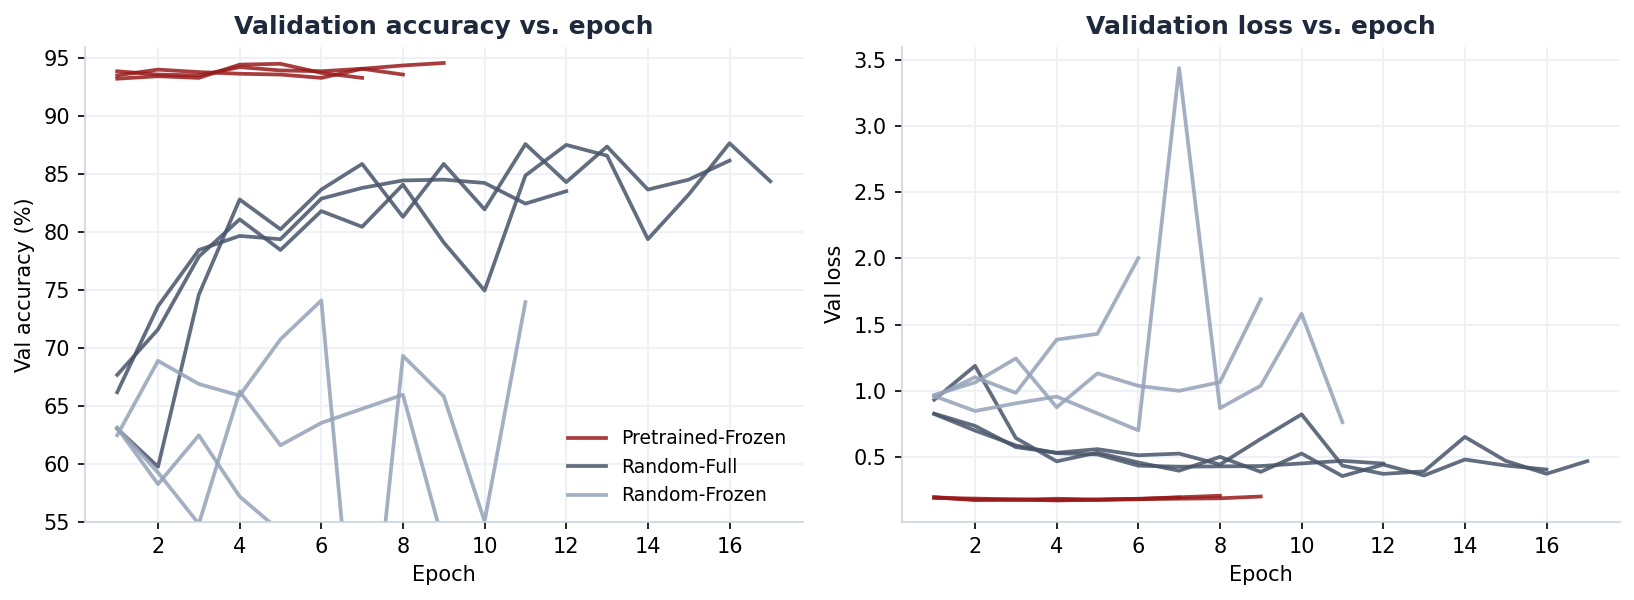
\includegraphics[width=0.98\textwidth]{../results/learning_curves.png}
\caption{Per-epoch validation accuracy (left) and loss (right) for all three conditions across the three seeds. Pretrained-frozen (dark red) converges within a few epochs; random-full (slate) climbs slowly over many epochs; random-frozen (light) is noisy and plateaus low.}
\label{fig:curves}
\end{figure*}

\subsection{Feature-Space Separability}
To visualize \emph{why} pretrained features help, Figure~\ref{fig:pca} projects the 512-dimensional penultimate features of the test images onto their first two principal components. The pretrained-frozen features form clearly separated per-class clusters, and the residual overlaps (glacier/mountain/sea, and buildings/street) mirror exactly the errors seen in the confusion matrix. The random-frozen features are largely entangled: the trainable head receives little linearly separable structure, which directly explains the large accuracy gap under matched capacity.

\begin{figure*}[t]
\centering
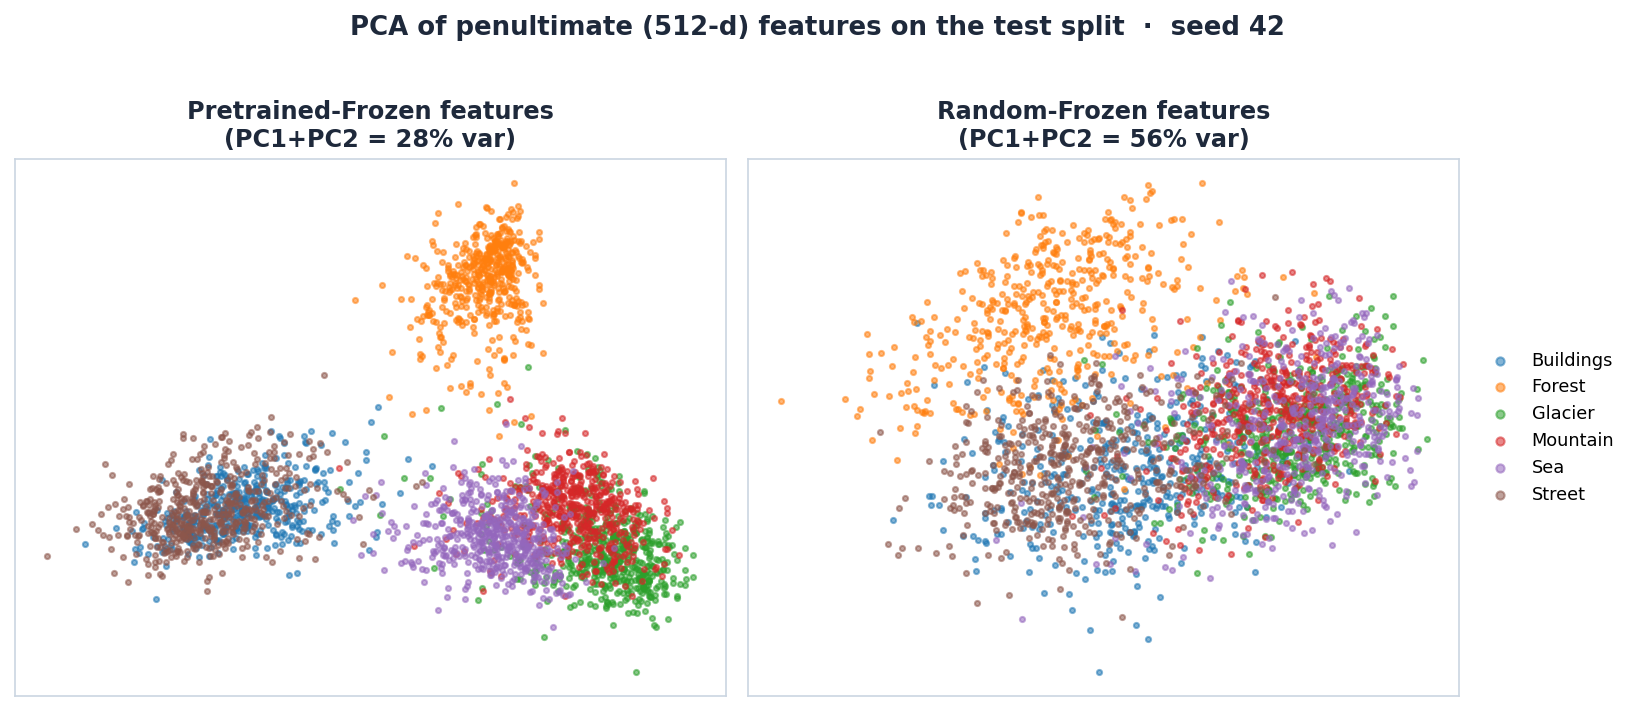
\includegraphics[width=0.98\textwidth]{../results/feature_pca.png}
\caption{PCA of penultimate (512-d) test features (seed 42). Pretrained-frozen features (left) separate the six classes; random-frozen features (right) remain entangled, with only forest partially separable.}
\label{fig:pca}
\end{figure*}

\subsection{Freeze-Depth Ablation}
\label{sec:ablation}
The three main conditions fix a single freeze boundary. To test how sensitive the result is to that choice, I sweep the boundary on the pretrained model: training only \texttt{fc} (a linear probe on frozen ImageNet features), then progressively unfreezing \texttt{layer4}, \texttt{layer3}, \texttt{layer2}, and finally the whole network. To keep the sweep tractable this ablation uses a fixed 40\% stratified subset of the training set at a single seed; the validation and test splits are unchanged, so accuracies are directly comparable within the sweep (and consequently sit slightly below the full-data numbers of Table~\ref{tab:test_acc}).

Figure~\ref{fig:ablation} shows the result. A bare linear probe already reaches 91.3\%, confirming that the frozen ImageNet features are highly linearly separable for this task. Unfreezing \texttt{layer4} adds about 1.6 points to 92.9\%, after which accuracy is flat: unfreezing \texttt{layer3}, \texttt{layer2}, or the full network yields 92.8\% each, while the trainable parameter count rises from roughly 3k to 11.2M with no accompanying benefit. This validates the partition used in the main experiments: training \texttt{layer4} plus the head captures essentially all of the attainable accuracy, and deeper fine-tuning only adds cost.

\begin{figure}[t]
\centering
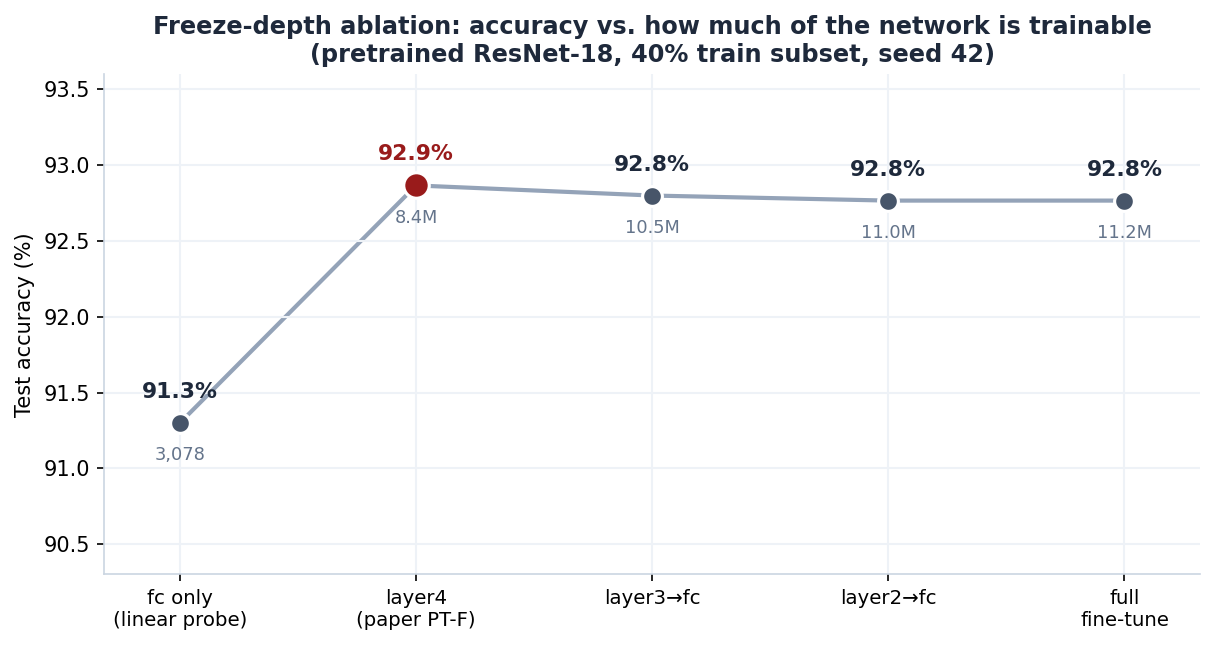
\includegraphics[width=\columnwidth]{../results/ablation_curve.png}
\caption{Test accuracy as the pretrained network is progressively unfrozen. Most of the benefit is already reached by a linear probe; training \texttt{layer4} (the boundary used in the main experiments) captures the rest; deeper fine-tuning adds nothing.}
\label{fig:ablation}
\end{figure}

\begin{table}[h]
\centering
\caption{Freeze-Depth Ablation (pretrained ResNet-18, 40\% train subset, seed 42)}
\label{tab:ablation}
\begin{tabular}{lccc}
\toprule
\textbf{Trainable from} & \textbf{Trainable Params} & \textbf{Test Acc.} & \textbf{Epochs} \\
\midrule
\texttt{fc} only (linear probe) & 3{,}078 & 91.30\% & 28 \\
\texttt{layer4} (main PT-F)     & 8.40M   & 92.87\% & 9 \\
\texttt{layer3}$\to$\texttt{fc} & 10.50M  & 92.80\% & 9 \\
\texttt{layer2}$\to$\texttt{fc} & 11.02M  & 92.77\% & 9 \\
Full fine-tune                  & 11.18M  & 92.77\% & 9 \\
\bottomrule
\end{tabular}
\end{table}

Table~\ref{tab:ablation} lists the corresponding numbers. Two features stand out: the linear probe needs many more epochs (28) to converge than any unfrozen variant (9), because only 3{,}078 parameters carry the entire adaptation; and once \texttt{layer4} is unfrozen, adding roughly 2.8M further trainable parameters (\texttt{layer3} through the full network) leaves test accuracy statistically unchanged. The chosen partition therefore sits exactly at the point of diminishing returns.

\subsection{First-Layer Substitution with Gabor Filters}
\label{sec:gabor}
The freeze-depth sweep asks how much of the pretrained network must adapt when the network is otherwise fixed. A sharper version of that question targets the \emph{first} layer specifically: if the learned first convolution is replaced by a fixed, hand-designed front end, how far up the network must weights re-adapt to compensate, and how much accuracy is permanently lost? Gabor filters are the classic hand-designed front end, long used as oriented edge and texture detectors~\cite{jain1991unsupervised}, and fixed wavelet front ends have been shown to rival learned first layers on some recognition tasks~\cite{bruna2013scattering}.

I replace ResNet-18's first convolution (\texttt{conv1}) with a fixed bank of 64 Gabor filters spanning 8 orientations, 4 wavelengths, and 2 phases (even and odd), and freeze it. Every other layer starts from ImageNet-pretrained weights. I then run the same freeze-depth sweep, unfreezing the residual stages as a growing prefix from the input side (\texttt{fc} read-out, then \texttt{+layer1}, \texttt{+layer2}, \texttt{+layer3}, and finally \texttt{+layer4}, i.e. everything except the frozen first conv), on the full training set at seed 42. As a matched reference I run the identical sweep with the ordinary learned \texttt{conv1} (also frozen). \texttt{bn1} and the head are trainable throughout so the fixed front end can be re-normalized and read out.

Figure~\ref{fig:gabor} shows both curves. With the learned first layer, a read-out already reaches 91.6\% and unfreezing more stages rises gently to 93.2\%. The Gabor front end behaves very differently. At read-out it scores only 81.1\%, roughly 10 points below the learned first layer, since a fixed Gabor \texttt{conv1} produces activations the pretrained upper layers were never built for. Unfreezing the single next stage (\texttt{layer1}) recovers most of that gap, jumping to 86.1\% ($+5.0$ points). After that the curve is essentially flat: \texttt{+layer2}, \texttt{+layer3}, and \texttt{+layer4} give 86.2\%, 86.6\%, and 86.3\%, so unfreezing anything beyond \texttt{layer1} makes almost no difference.

\begin{figure}[t]
\centering
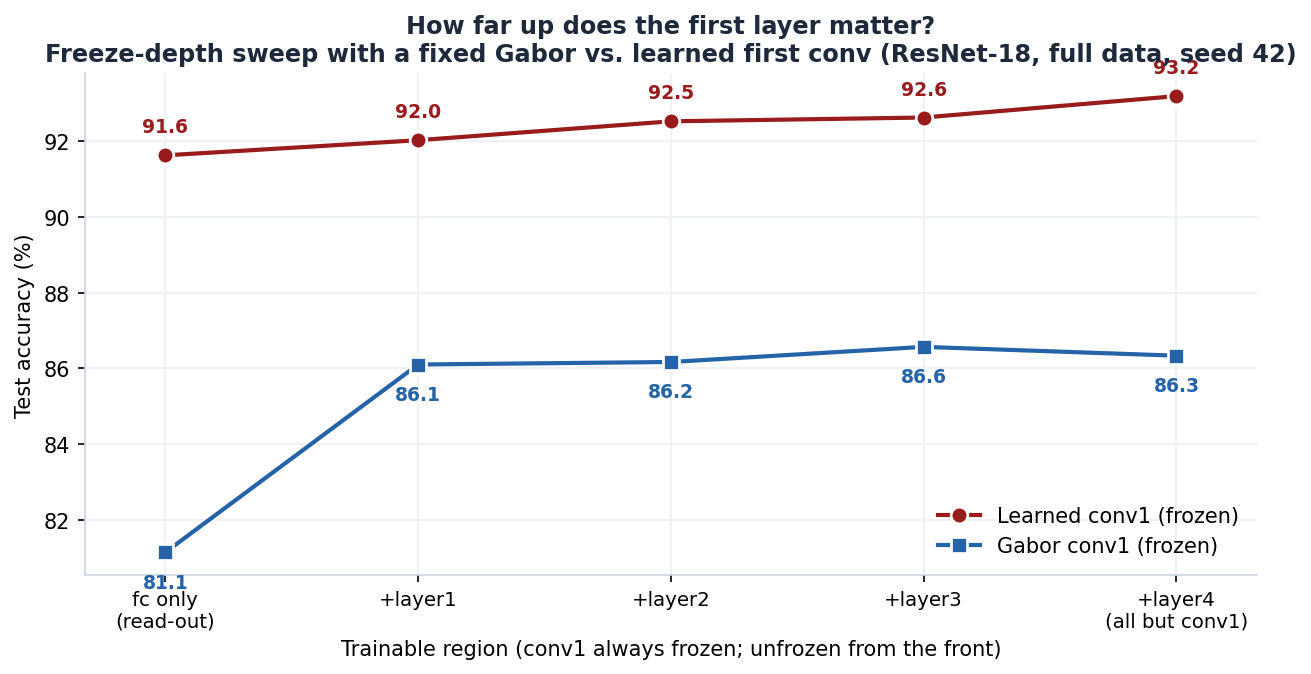
\includegraphics[width=\columnwidth]{../results/gabor_curve.png}
\caption{Freeze-depth sweep with a fixed Gabor first layer versus the learned first layer (both frozen; ResNet-18, full data, seed 42). Swapping in Gabor filters costs about 10 points at read-out; re-adapting only \texttt{layer1} recovers most of it, and unfreezing deeper stages adds almost nothing, so the first-layer influence reaches only about one stage up. A gap of roughly 7 points to the learned first layer persists even at full trainability.}
\label{fig:gabor}
\end{figure}

Two conclusions follow. First, the disturbance introduced by swapping the first layer is absorbed almost entirely by re-adapting the immediately following stage; its influence does not propagate more than about one stage up the network, because letting deeper stages adapt buys nothing. Second, the substitution leaves a persistent gap of roughly 7 points (86.3\% versus 93.2\%) even when every layer above \texttt{conv1} is trainable and the two runs have identical trainable capacity. The learned first-layer filters therefore carry information that a fixed Gabor bank plus unrestricted downstream retraining cannot reconstruct, a concrete measure of how much the first layer alone contributes on this task.

\section{Discussion and Summary}
\subsection{Isolating Pretraining Quality}
\label{subsec:quality}
PT-F and R-F share the same trainable parameters and the same freeze boundary, so the gap between them is down to feature quality alone. Table~\ref{tab:test_acc} shows that gap is large: 26.7 points of test accuracy on average (\pretrainedfrozenTestAccMean\ against \randomfrozenTestAccMean). Since $\theta_f$ in R-F is random and never updated, \texttt{layer4} has to turn essentially arbitrary patterns into class scores, which caps how far it can generalize. Even so, R-F reaches 66.5\%, well above the 16.7\% chance rate for six classes. That fits the findings of Jarrett et al.~\cite{jarrett2009best} and Saxe et al.~\cite{saxe2011random} that random convolutional filters still carry some frequency- and orientation-selective structure through pooling, so the random frozen extractor is a real baseline, not pure noise. PT-F, by contrast, starts from ImageNet weights that already encode edges, textures, and shape boundaries, and those features carry over well to the natural scenes in the Intel set.

\subsection{Isolating Trainable Capacity}
R-F and R-FL both start from random weights, so the gap between them is about capacity. R-FL can adapt every parameter, including $\theta_f$, so its early layers learn filters from the pixels up to fit the data instead of being stuck at their initial values. That lifts its mean accuracy to \randomfullTestAccMean, against the restricted \randomfrozenTestAccMean\ of R-F.

That recovers 18.1 points through capacity alone, appreciably less than the 26.7 points attributable to feature quality in Section~\ref{subsec:quality}. Both factors matter; the representation matters considerably more.

R-FL also takes much longer to train, converging in a mean of \randomfullValEpochsMean\ epochs against \randomfrozenValEpochsMean\ for R-F, and it still finishes 8.6 points short of PT-F at roughly four times the wall-clock cost. So extra capacity helps, but it cannot make up for a poor starting point when the data and the epoch budget are limited.

\subsection{Class-wise Confusions}
My test confusion matrices show consistent patterns of category-specific confusion across all conditions, though the errors are far more pronounced in the random initialization models. 
The primary confusion occurs between:
\begin{itemize}
    \item \textbf{Glacier vs. Mountain:} Visual features such as white snow, jagged ridges, and rock textures are shared heavily between these classes.
    \item \textbf{Buildings vs. Street:} Images of streets frequently contain buildings in the background, and vice-versa, making the spatial context highly overlapping.
\end{itemize}
These errors come from genuine visual overlap in the data, not from anything in the training setup.

\subsection{Limitations and Future Work}
A few things limit these conclusions.

\textbf{One dataset, one architecture.} I use one target dataset and one backbone (ResNet-18), so the 26.7-point figure is not claimed to generalize across domains or to deeper networks.

\textbf{Three seeds, no significance test.} The gaps between conditions far exceed the within-condition spread (Table~\ref{tab:test_acc}), but no formal significance test is run. The freeze-depth ablation of Section~\ref{sec:ablation} ran on a 40\% training subset at a single seed to save compute, and the Gabor substitution of Section~\ref{sec:gabor} reports a single seed on full data; both trends are clear, but tighter error bars would need several seeds. Read the shape of those two curves, not their exact values.

\textbf{No data augmentation.} The preprocessing pipeline is a single deterministic resize and centre crop shared by the training, validation, and test splits, with no random flips, crops, or colour jitter at training time. This was omitted deliberately to keep the three conditions on an identical input distribution, but it depresses absolute accuracy relative to tuned baselines and disadvantages R-FL in particular, since a fully trainable network is the arm that stands to gain most from augmentation. The comparison between conditions is unaffected; the absolute numbers should be read with this in mind.

\textbf{The Gabor bank is untuned.} Its orientations, wavelengths, and phases were fixed a priori rather than searched, so the residual 7-point gap in Section~\ref{sec:gabor} is an upper bound on the distance between a fixed oriented-filter front end and a learned one.

\textbf{The control is not a method.} Random-Frozen exists to hold capacity fixed. It is not a proposal for how to train anything, and its 66.5\% should not be read as a recommended configuration.

Every condition also shares one optimizer, learning rate, and early-stopping patience, so the comparison reflects a typical low-tuning setting rather than each method at its best.

The most useful next step is a data-fraction sweep. He et al.~\cite{he2019rethinking} argue that from-scratch training can match pretraining given enough data and iterations, so scaling the labeled set from a few hundred images up to the full split would show where, if anywhere, the two meet on scene classification. Running the ablation and the main comparison on a second backbone and a second dataset would show how far the ``most of the value needs almost no fine-tuning'' result carries. Repeating it on a domain far from ImageNet is the sharpest version of that test, since it is exactly the regime where Raghu et al.~\cite{raghu2019transfusion} found model size dominating rather than reused features. Two further extensions follow from the design: replacing the random control with a parameter-matched shallow network would separate depth from capacity, and sweeping the size of the pretraining corpus would show whether the 26.7-point gap grows or saturates.

\subsection{Summary}
The goal was to separate two things that a plain pretrained-versus-scratch comparison mixes together, and the capacity-matched control did that. With the trainable parameters held fixed, pretrained features are worth 26.7 points of test accuracy over random ones, against the 18.1 points that full trainable capacity buys on its own, and they converge in far fewer epochs. The supporting views agree: the learning curves show pretraining is useful almost from the first epoch rather than just ending higher, and the PCA shows why, with pretrained features falling into class-separable clusters while random frozen features stay mixed. The freeze-depth sweep adds a practical note, since a bare linear probe already recovers most of the accuracy, so on this task the benefit of pretraining needs almost no fine-tuning to reach. When data or compute is limited, starting from pretrained weights is the clear choice.

\section*{Acknowledgment}
The Gabor substitution of Section~\ref{sec:gabor} originated with Prof. Bruce Maxwell (CS 5330, Khoury College), whose question about how far the influence of the first layer reaches up the network became that experiment. The Intel Image Classification dataset is distributed publicly via Kaggle, and the ResNet-18 implementation and ImageNet-pretrained weights used throughout come from PyTorch and torchvision.

\section*{Supplementary Material}
\begin{sloppypar}
\noindent\textbf{Demo video.} A two-minute silent walkthrough with on-screen captions. The first segment runs the pretrained-frozen and random-frozen checkpoints over the same held-out test images side by side, showing the full softmax distribution for each; since both conditions train an identical 8{,}396{,}806 parameters, the disagreements are attributable to initialization alone. The second segment is a captioned pass over the result figures.\\
\url{https://drive.google.com/file/d/1JZSamG6WljxIDFxSjuwxOERkdl2lQ34F/view?usp=sharing}

\vspace{0.6em}
\noindent\textbf{Final presentation.}\\
\url{https://drive.google.com/file/d/1ImzhkgC75xF5Fq-7q1qQB8d4SKsGyZQx/view?usp=sharing}
\end{sloppypar}

\bibliographystyle{IEEEtran}
\bibliography{references}

\end{document}
